\documentclass{article}
\usepackage{listings}
\usepackage{graphicx}
\usepackage{pythonhighlight}
\title{Week2 Report}
\author{Zhang Heartbright}
\date{\today}
\usepackage[a4paper]{geometry}

\begin{document}
\maketitle
\tableofcontents
\newpage
\section{Forward Propagation in a deep Network}
    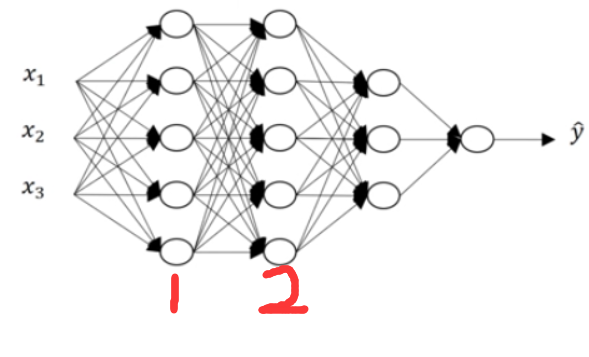
\includegraphics[width=10cm]{propagation.png}
    \subsection{Illustration}
    For the first layer we calculate X=$Z^[1]$=$W^[1]$x + $b^[1]$ \par
    then the activation for this layer is $a^[1]$=$g^[1]$($Z^[1]$) \par
    \par
    Then for the second layer we use $a^[1]$ as input, so we calculate :\par
    $Z^[2]$=$W^[2]$  $a^[1]$ +$b^[2]$ \par
    and so on ���� Use the former activation as the input for the current parameter
\newpage
\section{Building Blocks of deep neural Network}
    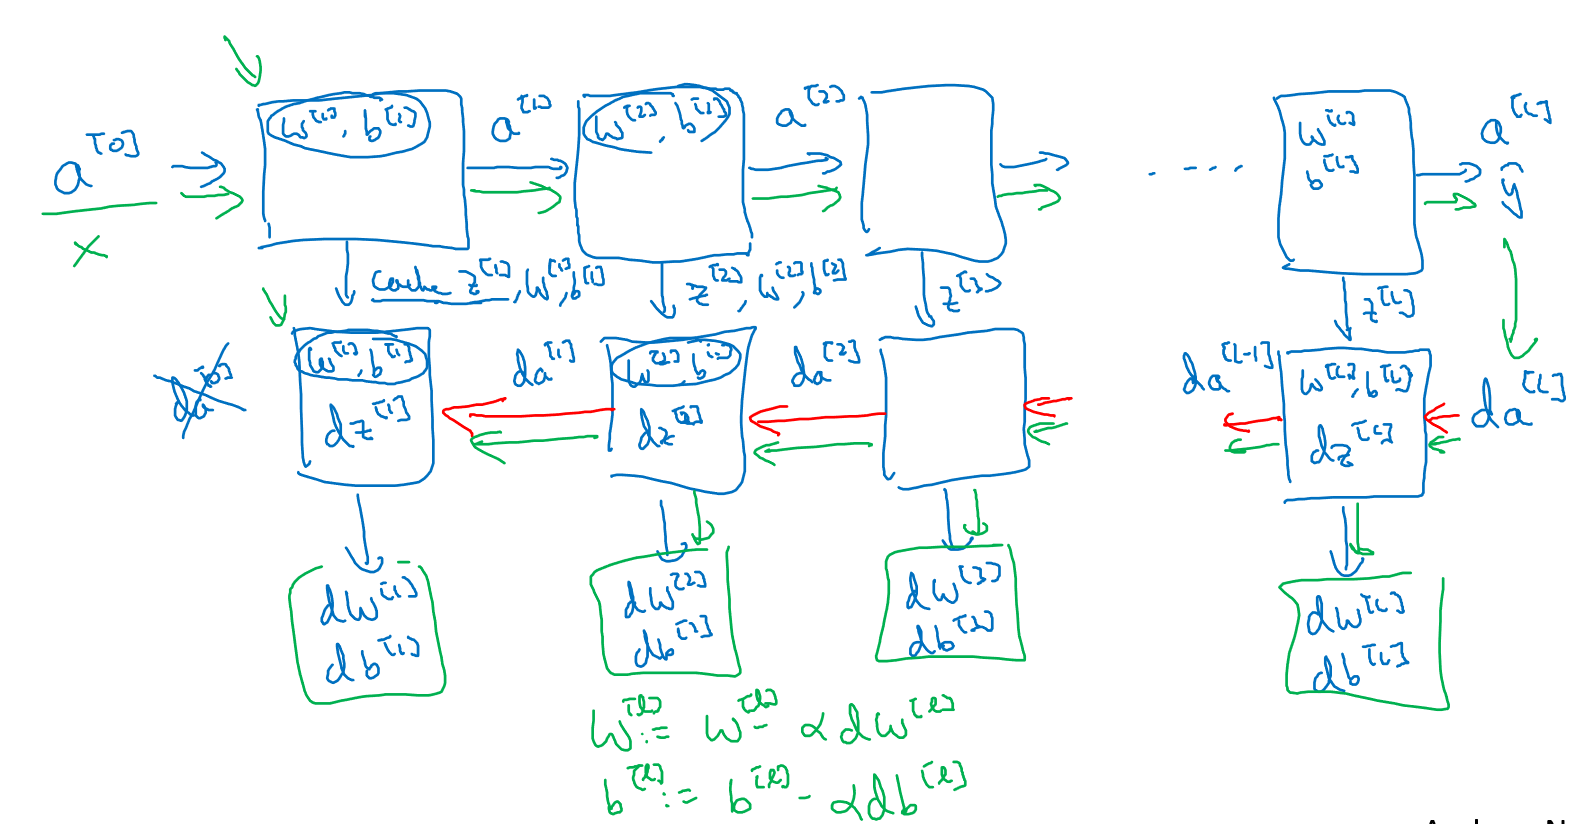
\includegraphics[width=10cm]{F_and_b_func.png}
    \subsection{}
    As the case in the picture, we input the feature $a^[0]$ ,we can propagate forward and calculate the activation which will used as the input of next layer\par
    For back propagating, use $\hat{y}$ to compute for $da^([l])$ and then get $dw^([l])$ and $db^([l])$
    and propagate back
\newpage
\section{Program for week2}
    \begin{abstract}
        I've struggled to fix my python3 and piped the scipy,h5py,matplot.\par
        It really challenging to practice. I didn't code it by myself, yet, I get through the meaning and learn the programmer of python.
    \end{abstract}
    \subsection{Codes}
    \begin{python}
import numpy as np
import matplotlib.pyplot as plt
import h5py
import scipy
from PIL import Image
from scipy import ndimage
from lr_utils import load_dataset

train_set_x_orig,train_set_y,test_set_x_orig,test_set_y,classes=load_dataset()

m_train=train_set_x_orig.shape[0]
m_test=test_set_x_orig.shape[0]
num_px=train_set_x_orig.shape[1]

train_set_x_flatten=train_set_x_orig.reshape(m_train,-1).T
test_set_x_flatten=test_set_x_orig.reshape(m_test,-1).T

train_set_x=train_set_x_flatten/255
test_set_x=test_set_x_flatten/255

def sigmoid(x):
    y=1/(1+(np.exp(-x)))
    return y

def initialize_with_zeros(dim):
    w=np.zeros([dim,1])
    b=0
    return w,b

def propagate(w,b,X,Y):
    m=X.shape[1]
    A=sigmoid(np.dot(w.T,X)+b)
    cost=(-1/m)*np.sum(np.multiply(Y,np.log(A))+np.multiply((1-Y),np.log(1-A)))
    dw=(1/m)*np.dot(X,(A-Y).T).T
    db=(1/m)*np.sum(A-Y)
    cost=np.squeeze(cost)
    grads={'dw':dw,'db':db}
    return grads,cost

def optimize(w,b,X,Y,num_iterations,learning_rate,print_cost=False):
    costs=[]
    for i in range(num_iterations):
        grads,cost=propagate(w,b,X,Y)
        dw=grads['dw']
        db=grads['db']

        w=w-learning_rate*dw.T
        b=b-learning_rate*db

        if i%100 ==0:
            costs.append(cost)

        if print_cost and i%100 == 0:
            print('Cost after iteration %i: %f'%(i,cost))

        params={'w':w,'b':b}
        grads={'dw':dw,'db':db}

    return params,grads,costs

def predict(w,b,X):
    m=X.shape[1]
    Y_prediction=np.zeros((1,m))
    w=w.reshape(X.shape[0],1)
    A=sigmoid(np.dot(w.T,X)+b)
    print(A)
    Y_prediction=np.around(A)
    print(Y_prediction)
    return Y_prediction

def model(X_train,Y_train,X_test,Y_test,num_iterations=2000,learning_rate=0.5,print_cost=False):

    w,b=initialize_with_zeros(X_train.shape[0])

    parameters,grads,costs=optimize(w,b,X_train,Y_train,num_iterations,learning_rate,print_cost);

    w=parameters['w']
    b=parameters['b']

    Y_prediction_test=predict(w,b,test_set_x)
    Y_prediction_train=predict(w,b,train_set_x)

    print("train accuracy: {} %".format(100 - np.mean(np.abs(Y_prediction_train - Y_train)) * 100))
    print("test accuracy: {} %".format(100 - np.mean(np.abs(Y_prediction_test - Y_test)) * 100))

    d = {"costs": costs,
         "Y_prediction_test": Y_prediction_test,
         "Y_prediction_train" : Y_prediction_train,
         "w" : w,
         "b" : b,
         "learning_rate" : learning_rate,
         "num_iterations": num_iterations}

    return d

learning_rates = [0.01, 0.001, 0.0001]
models = {}
for i in learning_rates:
    print ("learning rate is: " + str(i))
    models[str(i)] = model(train_set_x, train_set_y, test_set_x, test_set_y, num_iterations = 1500, learning_rate = i, print_cost = False)
    print ('\n' + "-------------------------------------------------------" + '\n')

for i in learning_rates:
    plt.plot(np.squeeze(models[str(i)]["costs"]), label= str(models[str(i)]["learning_rate"]))

plt.ylabel('cost')
plt.xlabel('iterations')

legend = plt.legend(loc='upper center', shadow=True)
frame = legend.get_frame()
frame.set_facecolor('0.90')
plt.show()
    \end{python}
    \subsection{Result}
    \begin{python}
    ######################################
    learning rate is: 0.01
[[0.97125943 0.9155338  0.92079132 0.96358044 0.78924234 0.60411297
  0.01179527 0.89814048 0.91522859 0.70264065 0.19380387 0.49537355
  0.7927164  0.85423431 0.00298587 0.96199699 0.01234735 0.9107653
  0.13661137 0.01424336 0.96894735 0.1033746  0.00579297 0.86081326
  0.53811196 0.64950178 0.83272843 0.00426307 0.0131452  0.99947804
  0.11468372 0.82182442 0.69611733 0.4991522  0.67231401 0.01728165
  0.04136099 0.80069693 0.26832359 0.03958566 0.74731239 0.32116434
  0.71871197 0.01205725 0.96879962 0.62310364 0.17737126 0.98960523
  0.74697265 0.07284605]]
[[1. 1. 1. 1. 1. 1. 0. 1. 1. 1. 0. 0. 1. 1. 0. 1. 0. 1. 0. 0. 1. 0. 0. 1.
  1. 1. 1. 0. 0. 1. 0. 1. 1. 0. 1. 0. 0. 1. 0. 0. 1. 0. 1. 0. 1. 1. 0. 1.
  1. 0.]]
[[1.47839653e-01 5.78008189e-02 9.42385025e-01 4.14849242e-05
  2.27209941e-02 7.29254667e-02 2.23704495e-02 9.49717864e-01
  5.41724297e-02 2.92729896e-02 6.82412299e-02 8.33370210e-01
  1.71420615e-01 9.66879883e-01 8.11537151e-01 2.44343486e-02
  7.87634096e-03 2.64027273e-02 5.60720048e-02 9.53130353e-01
  5.30865327e-03 3.11020747e-02 1.43606493e-01 1.92650472e-02
  9.30132798e-01 8.95291211e-01 2.72790551e-02 9.01480142e-01
  2.73987903e-02 8.09041583e-01 6.64266070e-02 5.00479730e-02
  1.29245158e-01 1.40274640e-01 6.48179132e-02 1.35261337e-02
  4.77693626e-03 2.65922709e-02 8.89771230e-01 2.64826222e-01
  1.22921586e-02 6.03229153e-01 8.81822076e-01 1.35079743e-02
  2.49595286e-02 6.88961129e-02 5.86046929e-02 8.68932415e-01
  5.14520332e-03 1.21099845e-02 8.23403970e-01 1.70985647e-01
  9.49977563e-02 3.04227660e-01 9.48091298e-01 8.09204742e-04
  9.66640038e-01 8.78319466e-01 3.17284881e-02 9.76165700e-01
  8.81584697e-01 8.48145722e-01 2.70795161e-02 2.28390395e-02
  1.05295676e-01 4.45165292e-02 1.22858876e-02 1.35813814e-01
  8.25867437e-01 9.21552659e-03 2.49353831e-02 9.88067070e-01
  5.78381495e-02 8.57292850e-02 4.10128551e-02 5.70507956e-01
  2.11603230e-04 1.52264723e-02 6.18390723e-02 1.39187810e-01
  6.68993749e-02 4.14281787e-04 1.23347661e-02 9.24789062e-01
  8.16880995e-01 9.29503653e-03 8.23770892e-02 2.75905820e-02
  8.52215781e-01 2.36580783e-02 1.75344552e-01 6.15499363e-02
  6.58017001e-01 9.54697511e-01 9.62775471e-01 1.05372217e-01
  9.37239410e-02 9.29062266e-01 2.68654455e-02 1.44668290e-01
  9.15662945e-02 2.89260931e-02 8.02603133e-01 6.11847788e-02
  9.87937141e-01 5.84677167e-02 9.87171184e-01 8.37167548e-01
  8.94717386e-01 8.58260204e-01 9.36232298e-01 9.33067878e-01
  8.77279898e-03 5.88387682e-02 5.09517612e-02 2.40626782e-02
  3.87480260e-02 9.35343373e-01 2.35202640e-03 8.83972092e-02
  4.49639007e-03 6.64404296e-01 1.76677024e-02 2.75426444e-05
  8.71728805e-01 2.43292079e-03 8.92351131e-01 9.50411302e-02
  9.66495010e-01 9.27285472e-01 2.66413779e-01 8.70883113e-02
  5.40743543e-02 9.75155427e-01 8.02323751e-01 6.92965781e-01
  9.06287458e-01 9.39900204e-01 1.64790717e-03 1.91364331e-02
  1.66925680e-02 1.46846280e-02 9.39237710e-01 2.57925925e-03
  8.19134438e-01 8.54311895e-01 9.10765300e-01 1.20452015e-01
  9.10603560e-01 9.11977137e-01 3.72174950e-01 6.13527932e-02
  1.30882744e-02 9.55225821e-01 4.30680817e-02 1.37970158e-01
  9.60868956e-01 8.67705031e-03 5.95741914e-03 2.19466775e-02
  1.78308410e-03 2.57658926e-02 8.63787547e-01 3.44218953e-02
  9.34152347e-01 9.35483280e-03 9.90908018e-01 1.17832721e-02
  2.67756873e-02 7.74546159e-01 8.43831858e-01 9.38847463e-01
  1.48599255e-01 4.17198955e-03 9.81043189e-01 8.22764984e-01
  1.92120395e-02 8.58870443e-01 5.37478572e-02 7.84878423e-01
  3.56080495e-02 2.80545015e-02 1.09777937e-02 1.30396160e-02
  3.81067987e-04 8.51025983e-01 2.44476493e-02 4.57657710e-02
  8.81871553e-01 1.06481929e-02 2.84032918e-02 1.96773462e-02
  8.54577180e-01 3.01055582e-02 1.33843958e-03 7.04152763e-02
  3.08344786e-01 9.25167630e-01 4.53183034e-02 9.31980530e-03
  8.69872444e-01 4.61339722e-03 4.86286964e-03 7.32772400e-03
  1.26009269e-01 1.46124056e-01 4.51019669e-02 1.45139959e-01
  1.45971589e-01]]
[[0. 0. 1. 0. 0. 0. 0. 1. 0. 0. 0. 1. 0. 1. 1. 0. 0. 0. 0. 1. 0. 0. 0. 0.
  1. 1. 0. 1. 0. 1. 0. 0. 0. 0. 0. 0. 0. 0. 1. 0. 0. 1. 1. 0. 0. 0. 0. 1.
  0. 0. 1. 0. 0. 0. 1. 0. 1. 1. 0. 1. 1. 1. 0. 0. 0. 0. 0. 0. 1. 0. 0. 1.
  0. 0. 0. 1. 0. 0. 0. 0. 0. 0. 0. 1. 1. 0. 0. 0. 1. 0. 0. 0. 1. 1. 1. 0.
  0. 1. 0. 0. 0. 0. 1. 0. 1. 0. 1. 1. 1. 1. 1. 1. 0. 0. 0. 0. 0. 1. 0. 0.
  0. 1. 0. 0. 1. 0. 1. 0. 1. 1. 0. 0. 0. 1. 1. 1. 1. 1. 0. 0. 0. 0. 1. 0.
  1. 1. 1. 0. 1. 1. 0. 0. 0. 1. 0. 0. 1. 0. 0. 0. 0. 0. 1. 0. 1. 0. 1. 0.
  0. 1. 1. 1. 0. 0. 1. 1. 0. 1. 0. 1. 0. 0. 0. 0. 0. 1. 0. 0. 1. 0. 0. 0.
  1. 0. 0. 0. 0. 1. 0. 0. 1. 0. 0. 0. 0. 0. 0. 0. 0.]]
train accuracy: 99.52153110047847 %
test accuracy: 68.0 %

-------------------------------------------------------

learning rate is: 0.001
[[0.74458179 0.63302701 0.70621076 0.7037801  0.5322598  0.43784581
  0.1843739  0.71778574 0.73717649 0.59122536 0.39837511 0.44491784
  0.63244572 0.53976962 0.09938522 0.7227688  0.12316033 0.58301417
  0.28145733 0.16609522 0.61461919 0.14166416 0.0865388  0.4251847
  0.67719513 0.61251308 0.46730808 0.11854922 0.21041046 0.8906756
  0.42313203 0.56013238 0.60322016 0.37148913 0.57460259 0.11968291
  0.24088599 0.65905854 0.4782032  0.14862075 0.4992436  0.61682528
  0.4795275  0.16260336 0.70722369 0.23929218 0.36719514 0.87223907
  0.45484261 0.19029187]]
[[1. 1. 1. 1. 1. 0. 0. 1. 1. 1. 0. 0. 1. 1. 0. 1. 0. 1. 0. 0. 1. 0. 0. 0.
  1. 1. 0. 0. 0. 1. 0. 1. 1. 0. 1. 0. 0. 1. 0. 0. 0. 1. 0. 0. 1. 0. 0. 1.
  0. 0.]]
[[0.34403391 0.18575705 0.63392388 0.00949352 0.185803   0.30979007
  0.13544854 0.75931407 0.18856286 0.16653711 0.47903517 0.55094252
  0.39894694 0.67613631 0.32941411 0.15120523 0.1515817  0.10868391
  0.21533234 0.78261458 0.09236643 0.13102179 0.30209379 0.22018859
  0.60467471 0.63089631 0.13786841 0.52162666 0.2229145  0.41807311
  0.20928386 0.22354737 0.51863273 0.37446655 0.12619979 0.24763606
  0.08217106 0.20570627 0.61668309 0.47341694 0.07578526 0.20272218
  0.63694514 0.17332725 0.12774778 0.38987251 0.25716102 0.57589232
  0.03660729 0.23627192 0.5058546  0.44851881 0.26882028 0.54506441
  0.63427748 0.07593065 0.79389128 0.55848777 0.20399827 0.82950311
  0.67551516 0.49340246 0.12825017 0.19483707 0.30405843 0.25239064
  0.23849329 0.28306742 0.39562206 0.1338017  0.20953382 0.84559705
  0.25983452 0.43347997 0.25869745 0.5275365  0.01851016 0.18226072
  0.11686925 0.24360522 0.11457144 0.09711829 0.11403479 0.64158072
  0.56492264 0.14249209 0.26621215 0.23562087 0.63347539 0.19718838
  0.41665293 0.2560914  0.20511226 0.75854285 0.62700096 0.22437352
  0.24158168 0.58986637 0.18250551 0.31168748 0.40230892 0.18766222
  0.37363736 0.24954905 0.81540625 0.33905562 0.85287524 0.46460165
  0.64873862 0.49476607 0.58689285 0.73160658 0.15974705 0.28192355
  0.21969254 0.17213348 0.24140747 0.59506433 0.09843999 0.4664941
  0.11789794 0.41615495 0.28828188 0.01549565 0.57657208 0.03491378
  0.56433333 0.52342054 0.58263447 0.828261   0.33112864 0.30054751
  0.13866344 0.7796039  0.49905825 0.23849455 0.65130553 0.54865883
  0.07475945 0.15289783 0.17277205 0.21093974 0.77996081 0.05731401
  0.43542011 0.62528802 0.58301417 0.39592429 0.62711359 0.62164606
  0.52142034 0.2237536  0.11263677 0.69875451 0.13460421 0.59843604
  0.62542932 0.06223702 0.08147044 0.16677973 0.0471795  0.29026597
  0.53465382 0.37298272 0.67567251 0.08157721 0.80300364 0.36035876
  0.12411481 0.3216639  0.50044148 0.71061923 0.38536321 0.15865892
  0.73153708 0.60089581 0.19123039 0.60169201 0.21145324 0.35174627
  0.1036799  0.15432715 0.08266478 0.1765554  0.0315303  0.4005418
  0.12684962 0.13818573 0.69657105 0.10353719 0.15229696 0.170385
  0.39005657 0.21251557 0.03788715 0.32853945 0.47339083 0.62631301
  0.22739755 0.0902158  0.56782331 0.17507791 0.20252309 0.09500011
  0.34504767 0.39618939 0.25822558 0.24550552 0.30677401]]
[[0. 0. 1. 0. 0. 0. 0. 1. 0. 0. 0. 1. 0. 1. 0. 0. 0. 0. 0. 1. 0. 0. 0. 0.
  1. 1. 0. 1. 0. 0. 0. 0. 1. 0. 0. 0. 0. 0. 1. 0. 0. 0. 1. 0. 0. 0. 0. 1.
  0. 0. 1. 0. 0. 1. 1. 0. 1. 1. 0. 1. 1. 0. 0. 0. 0. 0. 0. 0. 0. 0. 0. 1.
  0. 0. 0. 1. 0. 0. 0. 0. 0. 0. 0. 1. 1. 0. 0. 0. 1. 0. 0. 0. 0. 1. 1. 0.
  0. 1. 0. 0. 0. 0. 0. 0. 1. 0. 1. 0. 1. 0. 1. 1. 0. 0. 0. 0. 0. 1. 0. 0.
  0. 0. 0. 0. 1. 0. 1. 1. 1. 1. 0. 0. 0. 1. 0. 0. 1. 1. 0. 0. 0. 0. 1. 0.
  0. 1. 1. 0. 1. 1. 1. 0. 0. 1. 0. 1. 1. 0. 0. 0. 0. 0. 1. 0. 1. 0. 1. 0.
  0. 0. 1. 1. 0. 0. 1. 1. 0. 1. 0. 0. 0. 0. 0. 0. 0. 0. 0. 0. 1. 0. 0. 0.
  0. 0. 0. 0. 0. 1. 0. 0. 1. 0. 0. 0. 0. 0. 0. 0. 0.]]
train accuracy: 88.99521531100478 %
test accuracy: 64.0 %

-------------------------------------------------------

learning rate is: 0.0001
[[0.45098635 0.48539489 0.40959087 0.44864257 0.32818894 0.43729766
  0.28884626 0.46438078 0.45494399 0.45491705 0.36938309 0.41863679
  0.45816519 0.5031755  0.2842568  0.45155065 0.30672371 0.37824086
  0.26505548 0.27737934 0.40677576 0.28781555 0.24304775 0.38397796
  0.50642581 0.47047843 0.35358916 0.31561491 0.39430714 0.4603235
  0.37998879 0.3764821  0.32056264 0.38693085 0.40764828 0.23150119
  0.311659   0.44981144 0.43152263 0.26276732 0.37785575 0.48883282
  0.37790798 0.30969512 0.47842906 0.32857529 0.34457076 0.60547775
  0.40733226 0.28828383]]
[[0. 0. 0. 0. 0. 0. 0. 0. 0. 0. 0. 0. 0. 1. 0. 0. 0. 0. 0. 0. 0. 0. 0. 0.
  1. 0. 0. 0. 0. 0. 0. 0. 0. 0. 0. 0. 0. 0. 0. 0. 0. 0. 0. 0. 0. 0. 0. 1.
  0. 0.]]
[[0.4225819  0.31692389 0.42964509 0.14896683 0.28783033 0.38652698
  0.29492571 0.44991522 0.31988018 0.32391139 0.39318147 0.34804173
  0.40099138 0.31694856 0.28102266 0.3231201  0.25486297 0.18485428
  0.31900054 0.52941528 0.25568417 0.27297382 0.29762542 0.35834172
  0.38912252 0.4552143  0.2555983  0.34830216 0.29078565 0.27432926
  0.31094887 0.44330557 0.47172673 0.39765449 0.22386371 0.46108148
  0.27055987 0.31333951 0.49901097 0.439851   0.23953174 0.29809115
  0.42197081 0.28385499 0.2465556  0.40478121 0.35487343 0.45521241
  0.1451398  0.37485678 0.36671611 0.37909623 0.30298036 0.40151709
  0.40460677 0.24757226 0.50122617 0.38917296 0.3687779  0.50666786
  0.52492017 0.37864634 0.24031899 0.30627306 0.35114005 0.37398054
  0.43104844 0.31851314 0.37029232 0.29232461 0.37616632 0.52373453
  0.32507684 0.48381803 0.39170698 0.38646363 0.17397111 0.31623794
  0.24714356 0.35235176 0.17699762 0.33409149 0.3249697  0.49338319
  0.413497   0.25575577 0.31724095 0.36456893 0.45018347 0.34698807
  0.38500817 0.46053573 0.23091555 0.47268593 0.43291929 0.26828088
  0.30258929 0.4164904  0.24453098 0.27111067 0.39272427 0.3043153
  0.27984468 0.39085873 0.52409691 0.34966557 0.55950717 0.37739831
  0.43697184 0.33557455 0.38439647 0.48607992 0.30731772 0.31028645
  0.30037443 0.29400226 0.42714997 0.42909528 0.30432821 0.5227302
  0.32144602 0.4066469  0.43683178 0.17768611 0.4354696  0.18662466
  0.39558874 0.48819809 0.35425959 0.57279833 0.35098941 0.33429763
  0.31014998 0.49175402 0.44154511 0.31203466 0.38776576 0.38352489
  0.29611222 0.36104647 0.33824864 0.37198268 0.52831432 0.25732676
  0.36743298 0.44902822 0.37824086 0.36790056 0.41246464 0.37833397
  0.3418507  0.30119593 0.2592477  0.46753926 0.26777792 0.43134603
  0.32491304 0.19700069 0.25937972 0.33143626 0.19820128 0.35468513
  0.36334932 0.51823778 0.37235121 0.27650473 0.47271147 0.44760504
  0.33240186 0.29967323 0.41157608 0.47817969 0.39048545 0.28309008
  0.46350184 0.41099669 0.34508275 0.4323286  0.35065016 0.33976266
  0.25459527 0.29233107 0.26976618 0.30004182 0.18212017 0.34254174
  0.26213135 0.2674514  0.45817075 0.24356149 0.25227369 0.34588203
  0.3783451  0.32762257 0.19831251 0.51451759 0.3792938  0.41417054
  0.34795587 0.25521854 0.42313521 0.32557428 0.38342989 0.21943589
  0.34909483 0.39399177 0.36128874 0.38042346 0.38929593]]
[[0. 0. 0. 0. 0. 0. 0. 0. 0. 0. 0. 0. 0. 0. 0. 0. 0. 0. 0. 1. 0. 0. 0. 0.
  0. 0. 0. 0. 0. 0. 0. 0. 0. 0. 0. 0. 0. 0. 0. 0. 0. 0. 0. 0. 0. 0. 0. 0.
  0. 0. 0. 0. 0. 0. 0. 0. 1. 0. 0. 1. 1. 0. 0. 0. 0. 0. 0. 0. 0. 0. 0. 1.
  0. 0. 0. 0. 0. 0. 0. 0. 0. 0. 0. 0. 0. 0. 0. 0. 0. 0. 0. 0. 0. 0. 0. 0.
  0. 0. 0. 0. 0. 0. 0. 0. 1. 0. 1. 0. 0. 0. 0. 0. 0. 0. 0. 0. 0. 0. 0. 1.
  0. 0. 0. 0. 0. 0. 0. 0. 0. 1. 0. 0. 0. 0. 0. 0. 0. 0. 0. 0. 0. 0. 1. 0.
  0. 0. 0. 0. 0. 0. 0. 0. 0. 0. 0. 0. 0. 0. 0. 0. 0. 0. 0. 1. 0. 0. 0. 0.
  0. 0. 0. 0. 0. 0. 0. 0. 0. 0. 0. 0. 0. 0. 0. 0. 0. 0. 0. 0. 0. 0. 0. 0.
  0. 0. 0. 1. 0. 0. 0. 0. 0. 0. 0. 0. 0. 0. 0. 0. 0.]]
train accuracy: 68.42105263157895 %
test accuracy: 36.0 %
    ######################################
    \end{python}
    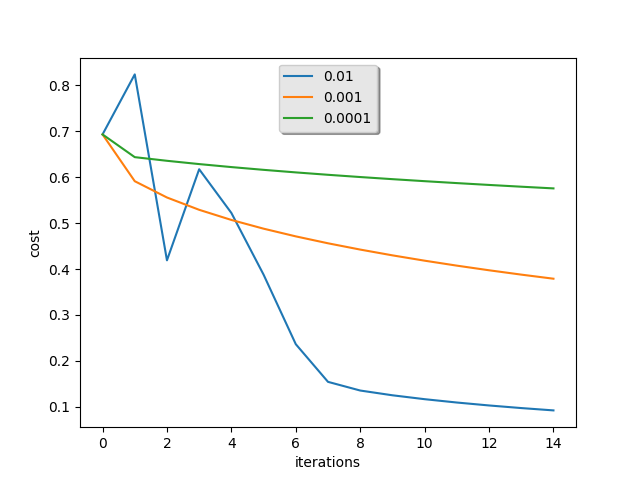
\includegraphics[width=10cm]{Figure_1.png}
\end{document}